\part{Zend Engine}


\chapter{Overview}


\section{Zend Engine1}

从性能或功能方面很容易到达PHP的瓶颈导致了Zend Engine1的开发,并且以Zend Engine1为基础开发了PHP4。

Zend是语言引擎,也是PHP内核,PHP是从外层展现的完整系统。

为了实现一个 web 脚本解释器,需要实现三个部分:

\begin{compactenum}
\item 解释器部分:分析输入代码,翻译代码,然后执行代码。
\item 功能部分:完成语言的功能(函数等)。
\item 接口部分:与web通信等。
\end{compactenum}

Zend完全参与第一部分,部分参与第二部分,PHP参与第二部分和三部分,它们最终一起构成完整的PHP包。

\begin{figure}[htbp]
\centering
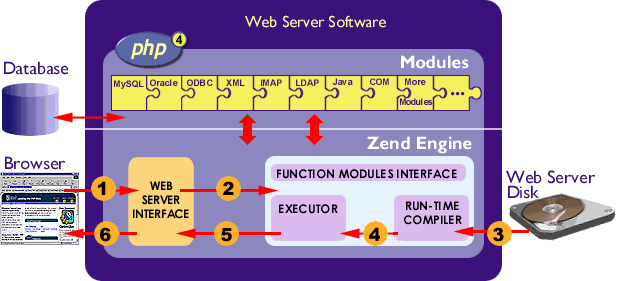
\includegraphics[scale=0.5]{internal-structure.png}
\caption{Web应用程序模型}
\end{figure}

PHP的主要组成部分包括外部扩展模块、内置模块和Zend Engine。其中,Zend Engine仅仅构成语言核心,并使用了预定义的函数来实现 PHP的非常基础的部分,PHP则包含所有的实际形成语言能力的所有模块。

\subsection{External Modules}

外部模块可以在脚本运行时使用dl()动态加载,具体来说就是dl()函数从磁盘加载一个共享的对象,并把它的功能提供给它被绑定的脚本。在脚本被终止后,外部模块将被从内存中丢弃。

外部模块不需要重新编译PHP,这样就可以让PHP文件保持很小的体积并且提供足够的功能,只是外部模块需要在每次请求时都重新加载并且在请求处理结束后立即卸载。

每一个需要使用外部模块提供的函数的PHP脚本都必须使用dl()函数或者在php.ini中的配置项来加载外部模块。

外部模块为使用PHP快速开发附加功能提供了最好的结果,在频繁使用和大型项目中其提供的好处大大抵消了频繁加载和代码复杂性的不足。

外部模块可以脱离PHP进行额外的配置,不需要重新编译PHP,PHP外部模块和PHP主模块完全分离的特性使得可以把应用程序方便地部署在生产环境中。

\subsection{Build-in Modules}

内置模块直接编译成PHP并且可以绑定到每个PHP进程中,因此内置模块提供的功能可以立即应用到正在运行的每个PHP脚本中。

内置模块无需动态加载,其提供的功能即时可用,而且内置模块本身都存储在PHP组件库中,只要内存足够就不会产生效率问题。

内置模块的每个修改都需要重新编译PHP,不过内置模块提供的函数库通常保持不变,这样就可以保持所有的PHP脚本的函数调用的可用性。





\section{Zend Engine2}



\section{Zend Engine3}




